\section{MicroNet}

MicroNet is a framework to develop and operate \ms{} applications. It is
designed to be especially support rich \ogs{}. MicroNet also provides all
needed to develop and operate an \og{}.

\subsection{Characteristics of MicroNet}

Microservices reduce the complexity of an online game by splitting the game
domain into small shards that can be developed independently. These shards are
defined by a domain driven design (DDD) approach.\\

How does MicroNet help in \og{} development:
\begin{itemize}
  \item MicroNet does not reinvent the wheel for online game development
  \item MicroNet works in conjunction with existing technologies, specifically popular game engines
  \item MicroNet tries to make the developer aware of the problems that are encountered during the development process
  \item While using MicroNet the developer learns the process of online game development 
  \item It helps the developers to get the difficult tasks like consistency of a
  asynchronous system right
\end{itemize}

What does MicroNet provide in this regard:
\begin{itemize}
  \item Provides a clear architecture for the game back-end
  \item Allows to develop individual game features independently
  \item Provides a simple protocol definition that helps the developers to loosely couple game features
  \item Offers standard solutions for technical requirements: Messaging
  functionality and Persistence functionality	
\end{itemize}

\subsection{Architecture Overview}

The MicroNet framework is a collection of components. Each component is
confined in itself which allows simple replacement of components. The components
are organized in three layers: The framework layer, the service catalogue layer,
and the tools layer. \autoref{fig:architecture_layers} shows the layers and all
the components they contain.

\begin{figure}
  \centering
  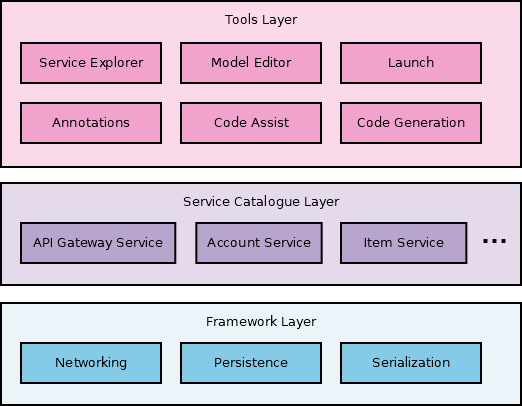
\includegraphics[width=0.7\textwidth]{images/architecture/ArchitectureLayers}
  \caption{The layered architecture of MicroNet with the associated components.}
  \label{fig:architecture_layers}
\end{figure}


The layers and the components they contain are explained below using Component
Responsibility Cards (CRC).

\newpage
\subsubsection{Framework Layer}

The framework layer provides a uniform interface to the core functionality of
MicroNet.\\

\noindent
\begin{tabular}{|l|l|}
    \cline{1-2}
    \multicolumn{2}{|c|}{} \\[-0.3cm]
    \multicolumn{2}{|c|}{Networking Component} \\ 
    \multicolumn{2}{|c|}{} \\[-0.3cm]
    \cline{1-2}
    Responsibility & Collaboration \\
    \cline{1-2}
    & \\[-0.2cm]
    \begin{minipage}{0.47\textwidth}
        \begin{itemize}
          \item Reliable Messaging System
          \item Connection Authentication
          \item Messaging API
        \end{itemize} 
    \end{minipage}
	&
    \begin{minipage}{0.47\textwidth}
        \begin{itemize}
          \item Message Broker (ActiveMQ)
          \item Serialization Component
        \end{itemize} 
    \end{minipage}
	\\ & \\
    \hline
\end{tabular}

\vspace{0.5cm} \noindent 
\begin{tabular}{|l|l|}
    \cline{1-2}
    \multicolumn{2}{|c|}{} \\[-0.3cm]
    \multicolumn{2}{|c|}{Persistence Component} \\ 
    \multicolumn{2}{|c|}{} \\[-0.3cm]
    \cline{1-2}
    Responsibility & Collaboration \\
    \cline{1-2}
    & \\[-0.2cm]
    \begin{minipage}{0.47\textwidth}
        \begin{itemize}
          \item Uniform Database Access
          \item Offer Relational Database 
          \item Offer NoSQL Database
          \item Java API
        \end{itemize} 
    \end{minipage}
	&
    \begin{minipage}{0.47\textwidth}
        \begin{itemize}
          \item Relational DBMS (PostgreSQL)
          \item JDBC
          \item NoSQL Database (Couchbase)
        \end{itemize} 
    \end{minipage}
	\\ & \\
    \hline
\end{tabular}

\vspace{0.5cm} \noindent 
\begin{tabular}{|l|l|}
    \cline{1-2}
    \multicolumn{2}{|c|}{} \\[-0.3cm]
    \multicolumn{2}{|c|}{Serialization Component} \\ 
    \multicolumn{2}{|c|}{} \\[-0.3cm]
    \cline{1-2}
    Responsibility & Collaboration \\
    \cline{1-2}
    & \\[-0.2cm]
    \begin{minipage}{0.47\textwidth}
        \begin{itemize}
          \item Uniform Serialization API
          \item Make serialization technology interchangeable
          \item Json serialization
          \item Binary serialization
        \end{itemize} 
    \end{minipage}
	&
    \begin{minipage}{0.47\textwidth}
        \begin{itemize}
          \item Serialization Library (Gson)
        \end{itemize} 
    \end{minipage}
	\\ & \\
    \hline
\end{tabular}

\subsubsection{Service Catalogue Layer}

The service catalogue was a mainly developed in the second semester thesis
\todo{Chapter 5 Prototype Implementation}. This section will exemplary give
three examples of catalogue services.\\

\noindent
\begin{tabular}{|l|l|}
    \cline{1-2}
    \multicolumn{2}{|c|}{} \\[-0.3cm]
    \multicolumn{2}{|c|}{API Gateway Service} \\ 
    \multicolumn{2}{|c|}{} \\[-0.3cm]
    \cline{1-2}
    Responsibility & Collaboration \\
    \cline{1-2}
    & \\[-0.2cm]
    \begin{minipage}{0.47\textwidth}
        \begin{itemize}
          \item Receive and filter requests from clients
          \item Forward requests to \mss{}
          \item Forward Events to clients
          \item Broadcast events to groups of clients
        \end{itemize} 
    \end{minipage}
	&
    \begin{minipage}{0.47\textwidth}
        \begin{itemize}
          \item Account Service (connection authentication)
        \end{itemize} 
    \end{minipage}
	\\ & \\
    \hline
\end{tabular}

\vspace{0.5cm} \noindent 
\begin{tabular}{|l|l|}
    \cline{1-2}
    \multicolumn{2}{|c|}{} \\[-0.3cm]
    \multicolumn{2}{|c|}{Account Service} \\ 
    \multicolumn{2}{|c|}{} \\[-0.3cm]
    \cline{1-2}
    Responsibility & Collaboration \\
    \cline{1-2}
    & \\[-0.2cm]
    \begin{minipage}{0.47\textwidth}
        \begin{itemize}
          \item User Registration
          \item User Authentication
        \end{itemize} 
    \end{minipage}
	&
    \begin{minipage}{0.47\textwidth}
        \begin{itemize}
          \item Account Database (PostgreSQL)
        \end{itemize} 
    \end{minipage}
	\\ & \\
    \hline
\end{tabular}

\vspace{0.5cm} \noindent 
\begin{tabular}{|l|l|}
    \cline{1-2}
    \multicolumn{2}{|c|}{} \\[-0.3cm]
    \multicolumn{2}{|c|}{Item Service} \\ 
    \multicolumn{2}{|c|}{} \\[-0.3cm]
    \cline{1-2}
    Responsibility & Collaboration \\
    \cline{1-2}
    & \\[-0.2cm]
    \begin{minipage}{0.47\textwidth}
        \begin{itemize}
          \item Player Inventory (Carried Items)
          \item Bank (Item Storage)
        \end{itemize} 
    \end{minipage}
	&
    \begin{minipage}{0.47\textwidth}
        \begin{itemize}
          \item Item Database (PostgreSQL)
        \end{itemize} 
    \end{minipage}
	\\ & \\
    \hline
\end{tabular}

\subsubsection{Tools Layer}

The development of the tool layer was a major part of the lab research. The
tools layer's main purpose is to provide aid with the tenet decentralized
continuous delivery. But the tools layer has also the responsibility to adapt
\ms{} application development to be suitable for \og{} development.\\

\noindent
\begin{tabular}{|l|l|}
    \cline{1-2}
    \multicolumn{2}{|c|}{} \\[-0.3cm]
    \multicolumn{2}{|c|}{Annotation Processing} \\ 
    \multicolumn{2}{|c|}{} \\[-0.3cm]
    \cline{1-2}
    Responsibility & Collaboration \\
    \cline{1-2}
    & \\[-0.2cm]
    \begin{minipage}{0.47\textwidth}
        \begin{itemize}
          \item Framework functionality\footnotemark 
          \item Boilerplate code reduction
          \item Defining the shared messaging API
        \end{itemize} 
    \end{minipage}
	&
    \begin{minipage}{0.47\textwidth}
        \begin{itemize}
          \item Shared Model (to export the API)
        \end{itemize} 
    \end{minipage}
	\\ & \\
    \hline
\end{tabular}

\footnotetext{The user code is
          called by the framework (application skeleton) opposed to the user
          code calling a library (well-defined operations).}
          
\vspace{0.5cm} \noindent      
\begin{tabular}{|l|l|}
    \cline{1-2}
    \multicolumn{2}{|c|}{} \\[-0.3cm]
    \multicolumn{2}{|c|}{Code Assist} \\ 
    \multicolumn{2}{|c|}{} \\[-0.3cm]
    \cline{1-2}
    Responsibility & Collaboration \\
    \cline{1-2}
    & \\[-0.2cm]
    \begin{minipage}{0.47\textwidth}
        \begin{itemize}
          \item Present the Shared API to the developer
          \item Auto-completion of URIs
          \item Recognize API usage errors at compile-time
        \end{itemize} 
    \end{minipage}
	&
    \begin{minipage}{0.47\textwidth}
        \begin{itemize}
          \item Shared Model (to import the API)
        \end{itemize} 
    \end{minipage}
	\\ & \\
    \hline
\end{tabular}

\vspace{0.5cm} \noindent         
\begin{tabular}{|l|l|}
    \cline{1-2}
    \multicolumn{2}{|c|}{} \\[-0.3cm]
    \multicolumn{2}{|c|}{Code Generation} \\ 
    \multicolumn{2}{|c|}{} \\[-0.3cm]
    \cline{1-2}
    Responsibility & Collaboration \\
    \cline{1-2}
    & \\[-0.2cm]
    \begin{minipage}{0.47\textwidth}
        \begin{itemize}
          \item Generate the MicroNet Framework integration classes
          \item Generate POJOs from the Shared Model
        \end{itemize} 
    \end{minipage}
	&
    \begin{minipage}{0.47\textwidth}
        \begin{itemize}
          \item Shared Model (to import the API and Template Types)
          \item Java compiler (annotation processing)
        \end{itemize} 
    \end{minipage}
	\\ & \\
    \hline
\end{tabular}

\vspace{0.5cm} \noindent         
\begin{tabular}{|l|l|}
    \cline{1-2}
    \multicolumn{2}{|c|}{} \\[-0.3cm]
    \multicolumn{2}{|c|}{Service Explorer} \\ 
    \multicolumn{2}{|c|}{} \\[-0.3cm]
    \cline{1-2}
    Responsibility & Collaboration \\
    \cline{1-2}
    & \\[-0.2cm]
    \begin{minipage}{0.47\textwidth}
        \begin{itemize}
          \item Management visual interface for the application (UI)
          \item Compose the application out of catalogue and developed game
          services
        \end{itemize} 
    \end{minipage}
	&
    \begin{minipage}{0.47\textwidth}
        \begin{itemize}
          \item Service Catalogue
          \item Launch Utility (to provide the UI)
        \end{itemize} 
    \end{minipage}
	\\ & \\
    \hline
\end{tabular}

\vspace{0.5cm} \noindent      
\begin{tabular}{|l|l|}
    \cline{1-2}
    \multicolumn{2}{|c|}{} \\[-0.3cm]
    \multicolumn{2}{|c|}{Model Editor} \\ 
    \multicolumn{2}{|c|}{} \\[-0.3cm]
    \cline{1-2}
    Responsibility & Collaboration \\
    \cline{1-2}
    & \\[-0.2cm]
    \begin{minipage}{0.47\textwidth}
        \begin{itemize}
          \item Define and edit the shared model as template types
          \item Instantiate templates as prefabs
          \item Synchronize the Shared Model between developers
        \end{itemize} 
    \end{minipage}
	&
    \begin{minipage}{0.47\textwidth}
        \begin{itemize}
          \item Shared Model (CRUD)
          \item Database Component (for sharing)
        \end{itemize} 
    \end{minipage}
	\\ & \\
    \hline
\end{tabular}

\vspace{0.5cm} \noindent        
\begin{tabular}{|l|l|}
    \cline{1-2}
    \multicolumn{2}{|c|}{} \\[-0.3cm]
    \multicolumn{2}{|c|}{Launch Utility} \\ 
    \multicolumn{2}{|c|}{} \\[-0.3cm]
    \cline{1-2}
    Responsibility & Collaboration \\
    \cline{1-2}
    & \\[-0.2cm]
    \begin{minipage}{0.47\textwidth}
        \begin{itemize}
          	\item Build the composed application
			\item Simplify application deployment
          	\item Provide launch configurations for local deployments 
        \end{itemize} 
    \end{minipage}
	&
    \begin{minipage}{0.47\textwidth}
        \begin{itemize}
          \item Maven (build)
          \item Docker (build \& run)
          \item Docker-compose (compose the application)
          \item optionally uses CDT Launch Groups and Eclipse Docker Tools
        \end{itemize} 
    \end{minipage}
	\\ & \\
    \hline
\end{tabular}

\subsection{Networking}
\label{sub:networking}
Networking in MicroNet has been discussed in detail in section 6.5 Networking
Implementation in project thesis one \cite{biedermann2015project1}. The original
implementation was improved in the course of all three theses and this section
provides a summary of the final implementation solution of networking.

Networking is the most fundamental aspect of an \og{} development and crucial
for the stability of \ms{} applications. The networking concept for \ms{}
applications is heavily influenced by the IDEAL tenet because it makes it
necessary to provide an abstract messaging concept that is decoupled from any
implementation.

In MicroNet this network abstraction is realized by defining a set of networking
capabilities that must be supported by the underlying network technology. These
capabilities are represented in the form of the \code{IPeer} Java interface
shown in \autoref{lst:ipeer_interface}. Standard services can therefore
communicate over an instantiation of the \code{IPeer} interface injected by the
framework. This makes the underlying technology exchangeable since the interface
is stable. This allows platform independence as long as the services are written
in Java.

\begin{figure}
	\begin{lstlisting}[language=Java,firstnumber=1] 
public interface IPeer {
	void startup(URI host);
	void shutdown();
	
	void sendRequest(URI destination, Request request);
	void sendRequest(URI destination, Request request, 
		Consumer<Response> handler);
		
	Response sendRequestBlocking(URI destination, Request request);
	Response sendRequestBlocking(URI destination, Request request,
		int timeout);
		
	void listen(String path, Consumer<Request> handler);
	void listen(String path, Function<Request, Response> handler);
}
	\end{lstlisting}
  	\caption{The iPeer interface must be implemented to participate in MicroNet
  	applications.}
  	\label{lst:ipeer_interface}
\end{figure}

MicroNet implements this networking interface by relying on ActiveMQ as a
message broker. Although it would be possible to replace ActiveMQ as the
MicroNet networking technology this is out of the scope of this thesis to be
validated in practice. As a result MicroNet is heavily dependent on ActiveMQ.

According to the polyglot programming tenet it is a requirement that arbitrary
technologies can participate in a \ms{} application despite the tight coupling
with ActiveMQ. To accomplish this an adapter must be implemented to couple the
foreign technology with the application. The adapter can be an
implementation of an equivalent messaging interface in another programming
language using one of the many proposed ways to integrate with ActiveMQ like
RESTful HTTP, JMS, .NET, C/C++, Go, Node.js, Python, and more.

For game engine integration the messaging interface also has to be implemented
in the respective technology of the engine. In the case of MicroNet ActiveMQ
Unity3D is used as the refernce game engine which is written in C\#. For this
purpose the NMS \gls{api} which is a .NET port of the Java Message Service (JMS)
interface is used to make MicroNet accessible from the Unity3D game engine.

\subsubsection{Messaging System}

Messaging in MicroNet evolves around patterns: API Gateway, Reverse Proxy and
Pipes and Filters.

MicroNet uses a reverse proxy to interchange messages from the public Internet
with the internal network used by MicroNet. For this purpose two separate
message brokers are used and only the public broker is exposed to the Internet.
The gateway intercepts all messages from the public network and forwards them to
the responsible \ms{}. This is further detailed in the Messaging \gls{api} section
below.

The reverse proxy in fact also is the API gateway. An API gateway is a standard
approach offering the \textit{Service API} to the users. Upon reception of a
message the gateway can filter it according to a white- or blacklisting approach.

\begin{figure}
\begin{lstlisting}[language=Java,firstnumber=1] 
@MessageService(uri = "mn://foo")
public class ServiceFoo {
	@OnStart
	public void onStart(Context context) {
		URI destination = URI.create("mn://bar/hello");
		Request request = new Request("Hello from Foo!");
		context.getPeer().sendRequest(destination, request, response -> {
			System.out.println("Received Response: " + response.getData());
		});
	}
}

@MessageService(uri = "mn://bar")
public class ServiceBar {
	@MessageListener(uri="/hello")
	public Response helloHandler(Context context, Request request) {
		System.out.println("Received Request: " + request.getData());
		return new Response(StatusCode.OK, "Likewise, Bar");
	}
}
\end{lstlisting}
\caption{Two MicroNet services communicating with each other.}
\label{lst:service_communication}
\end{figure}

\mss{} can access the messaging functionality by using the context object
injected by the framework. \autoref{lst:service_communication} shows an example
of two simple \mss{} communicating with each other. It has to be mentioned that
the two services in the listing are fully functional without any additional
code necessary. The setup of the context and the \ms{}'s main function are
completely abstracted by the framework.

\paragraph{Message Parameters}

One useful feature that MicroNet provides are typed message parameters. These
parameters are defined using Parameter Codes and the \textit{Template Types}
both defined int the \textit{Shared Model}.

Message parameters spare the developer the need to individually define a
specific payload for each message transfer. For example slightly different
messages can be distinguished by only using parameter codes and leaving the
payload unchanged.

\begin{figure}
\begin{lstlisting}[language=Java,firstnumber=1] 
@MessageService(uri = "mn://foo")
public class ServiceFoo {
	@OnStart
	public void onStart(Context context) {
		URI destination = URI.create("mn://bar/hello");
		Request request = new Request("Hello from Foo!");
		request.getParameters().set(ParameterCode.ID, 42);
		context.getPeer().sendRequest(destination, request);
	}
}

@MessageService(uri = "mn://bar")
public class ServiceBar {
	@MessageListener(uri="/hello")
	public void helloHandler(Context context, Request request) {
		int parameter = request.getParameters().getInt(ParameterCode.ID);
		System.out.println("Received Request with Parameter: " + parameter);
	}
}
\end{lstlisting}
\caption{Adding a parameter to a MicroNet message.}
\label{lst:message_parameters}
\end{figure}

\autoref{lst:message_parameters} shows how services can transmit parameters
along with a request. For responses this works exactly the same.

\subsubsection{Connection Authentication}

Security is always a concern in regard to Internet applications. The backbone
of distributed application security is user connection authentication.
Since multiple gateways can be active simultaneously the integrity of the user
has to be validated by the gateway with every request. The gateway validates the
user request by looking up the user connection in the session store and
comparing it to the connection the request was received from. If no user session
is present in the session store the user connection is considered
unauthenticated.

For unauthenticated connections the gateway only forwards login messages to the
login service. Upon a positive login response from the account service the
processing gateway adds the user connection to the session store. Other gateways
are then able to look up if a connection is authenticated. The advantage of this
solution is that it scales very well. The downside is that it involves many
reads of the session store.

A requirement for this approach to work is that the underlying networking
provides a way to correlate incoming messages with a connection. This can be
done generating a connection ID hash based upon the user's IP/port combination.
ActiveMQ has this capability already built in by providing a globally unique
connection ID per connection.

The connection authentication process is further explained in
\autoref{sub:session_management}.

\subsubsection{MicroNet Messaging API}

The messaging \gls{api} provided by a MicroNet applications is a direct implementation
of the fine-grained interfaces tenet. It offers the following functionality to
promote stateless message transfers:

\begin{itemize}
  \item Sending a request to a \ms{} either from a user or another \ms{}
  \item Sending a request to a \ms{} and waiting for a response with a
  short\footnote{5 - 15 seconds of timeout seem appropriate for most short
  requests.} timeout either from a user or another \ms{}
  \item Sending an event to a user from a \ms{}
  \item Sending an event to a group of users from a \ms{}
  \item Sending a message to a topic, meaning to all subscribed \mss{}
  \item Named message parameters
\end{itemize}

\begin{figure}
	\centering
	\hspace*{-1.5cm}
	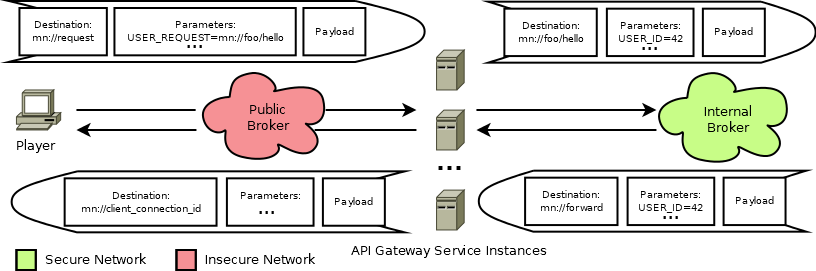
\includegraphics[width=1.2\textwidth]{images/architecture/MessagingAPI}
	\caption{The API Gateway offers the MicroNet messaging \gls{api} to the player.}
	\label{fig:messaging_api}
\end{figure}

These messaging capabilities are sufficient to model any arbitrary message
transfer. They leave a great degree of freedom and make message transfer
implementation very comfortable. 

\autoref{fig:messaging_api} shows the communication between a user and a
MicroNet application. The user in this scenario is already authenticated so the
gateway only needs filter client quests according to access restrictions. The
user sends his request to the \code{mn://request} queue which leads to an
arbitrary gateway instance consuming the request. The gateway reads the
\code{USER\_REQUEST} parameter from the request and according to it forwards the
message to the internal broker. Depending on the situation if the user expects a
response within the defined timeout or if no response is expected the
gateway holds on to a temporary response queue which allows immediate responses.
Such an immediate response can also indicate that the request will need longer
to be processed and therefore the requestor has to act accordingly and wait for
an asynchronous response.

These asynchronous responses are called events. An event can either be sent to a
single user or to a group of users. For this purpose \mss{} can send a request
to the \code{mn://forward} queue which is consumed by any gateway who in
response forwards the event to the corresponding user or group.

One last feature of the MicroNet messaging \gls{api} is the ability to send messages
to topics which can be subscribed by any service. This allows services to react
on events happening throughout the application. This can be for example the
\textit{new player connected} event.












\subsection{Composition Concepts}

The major challenge during the development of a \ms{} application is to achieve
loose coupling according to the IDEAL tenet. The goal of loose coupling is to
reduce dependencies among services. It has to be noticed that the coupling
between services can never be zero. Without any coupling the application cannot
function as a whole. MicroNet several basic concepts to reduce service coupling
while preserving reasonable development comfort. These concepts are discussed in
this section.

\subsubsection{Dependency Abstraction}

Dependency abstraction is a concept to reduce the number of dependencies
that \mss{} must explicitly add to the Java classpath to access core
functionality networking, persistence, and serialization.

According to the dependency abstraction concept external libraries are wrapped
within the core framework to offer standard access to the underlying dependency.
\mss{} can use the MicroNet wrapper libraries instead of using the
dependencies directly. This allows for exchangeability of the dependencies
without touching any \mss{} services. MicroNet integrates dependent libraries
into the wrapper libraries by the use of Maven which allows a very flexible
dependency chain. \autoref{fig:dependency_abstraction} shows which libraries are
abstracted by which framework component.

\begin{figure}
	\centering
	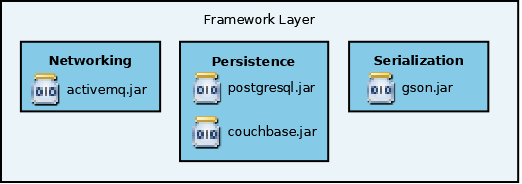
\includegraphics[width=10cm]{images/architecture/DependencyAbstraction}
	\caption{Dependency Abstraction in the MicroNet core framework.}
	\label{fig:dependency_abstraction}
\end{figure}

It has to be mentioned that the dependency abstraction layer is a dependency
itself and therefore it increases service coupling. But since the abstraction
layer unifies dependency access it helps to respect the don't repeat yourself (DRY)
principle and therefore increases overall cohesion of the application. 

Since the MicroNet adaption layer is realized using Java wrapper libraries,
this approach works very well for all Java \mss{} but none Java services have to
use the dependencies directly.

\subsubsection{Shared Model}
\label{subsub:shared_model}

The general design of how to incorporate a game model into a \mn{} application
is reclined to the design of modern game engines like Unity3D or UnrealEngine 4.
What these engines have in common is a graph to store the game state e.g. all
objects, levels, players, etc. This concept of game data organization will be
referred as the game graph. Two examples of game graphs are shown in
\autoref{fig:scenegraph}.

\begin{figure}
  \centering
  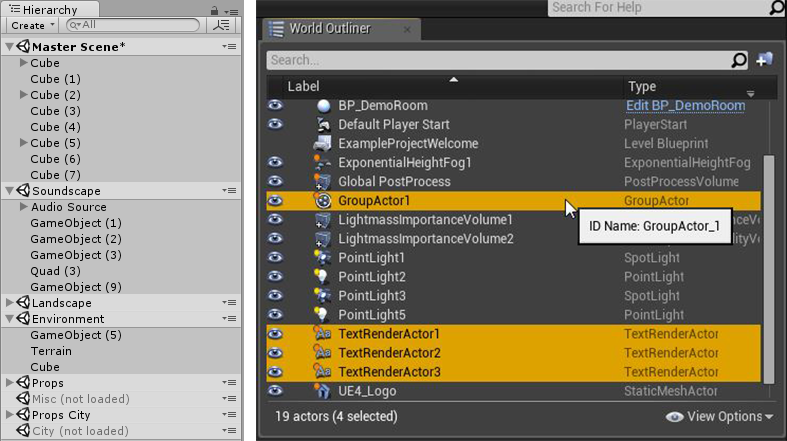
\includegraphics[width=\textwidth]{images/game_engine/scenegraph}
  \caption{Two example game graphs of the Unity3D (left) and the UnrealEngine4
  (right).}
  \label{fig:scenegraph}
\end{figure}

The shared model concept is mainly inspired by game graph concept of game
engines. The graph is represented by a Json document structure and can be shared
either using a git repository or by using a development database. The Json
format helps to achieve platform independence.

The shared model specifically allows to strongly type message transfers and
unifies database access. The design of the shared model allows to integrate the
game graph in a game engine because the concepts are closely related.

The shard model represents the game graph in the form of two individual trees:
The template tree and the prefab tree. The template tree is responsible to store
types. Types are templates to define all entities of the game. Entities are not
restricted to one purpose and can be used to store or transmit domain data.
Templates are plain data objects and can be thought as the equivalent to Java
POJOs. Momentarily it is not possible to add game logic to templates. But this
is planned for the future by using code injection (explained in
\autoref{sub:model_code_injection}). \autoref{lst:template_type} shows an
example of a template type in the template tree.

The types supported of the template tree are directly derived by the java types
because they work natively with the Java side of MicroNet. The Java types are
well documented in the Java language definition and can therefore be replicated
in other programming language to achieve deterministic behaviour on all systems.
The supported types are: STRING, NUMBER (INT, FLOAT, DOUBLE, \ldots), BOOLEAN, CHAR,
ENUM, LIST, SET, MAP, and COMPONENT. More information about the supported types
can be found in paragraph Model Editor in \autoref{sub:tools}.

\begin{figure}
\begin{lstlisting}[language=json,firstnumber=1] 
{
  "name": "UserValues",
  "variables": [
    {
      "name": "id",
      "type": {
        "numberType": "INT",
        "type": "NUMBER"
      }
    },
    {
      "name": "credentials",
      "type": {
        "componentType": "CredentialValues",
        "type": "COMPONENT"
      }
    }
  ]
}
\end{lstlisting}
\caption{The template type for the UserValues domain object in the template
tree.}
\label{lst:template_type}
\end{figure}

The second tree is the prefab tree. It is responsible to store actual instances
of templates representing the statical part of the game state. The prefab tree
is a concept to allow game designers to define the properties of the game in a
way which is directly understood by MicroNet and can therefore directly be used
to persist and synchronize the game. \autoref{lst:prefab_type} shows how a
prefab of the \code{UserValues} object looks like.

\begin{figure}
\begin{lstlisting}[language=json,firstnumber=1] 
{
  "id": 42,
  "credentials": {
    "username": "Jonas",
    "password": "1234"
  }
}
\end{lstlisting}
\caption{A prefab of the UserValues template type.}
\label{lst:prefab_type}
\end{figure}



\subsubsection{Service API}

The messaging system described in \autoref{sub:networking} is the main driver
for logical composition in MicroNet applications. The service API is offered to
the user by the API gateway in the form of a URI addressing. \mss{} can also use
this scheme to find each other internally. The only requirement to use the API
is to have access to the underlying message broker either trough the MicroNet
networking component or a direct connection to ActiveMQ.

The MicroNet service API is defined by using static URIs using the specific
form: \textit{ms://servicename/fine/grained/api}. The host portion of the URI is
used for participant discovery by using the message broker functionality to
register queues for the specific service address, \textit{ms://servicename} in
this example. The remainder of the URI, \textit{fine/grained/api} in this
example represents the fine grained service API defined by the \ms{} according
to tenet Fine-grained Interfaces. This Service API scheme of MicroNet is
inspired by a RESTful URI schema but is only static\footnote{Requests to URIs
like \textit{mn://player/123341214/some/functionality} are not realized}. Within
\mss{} the service API is defined using Java annotations described in paragraph
Annotations in \autoref{sub:tools}.

\subsubsection{Service Catalogue}

The service catalogue is a layer of MicroNet that uses the underlying framework
to provide reference service implementations for commonly requires
functionality. The service catalogue is realized by using Maven archetypes. An
archetype represents a skeleton or a basic implementation of a feature and can
be extended by the developer. It is possible for developers to contribute
services to a private service catalogue by creating a new Maven archetypes and
making them available for future reuse. \autoref{fig:service_catalogue} shows
how the service catalogue is integrated in the game development process.

\begin{figure}
	\centering
	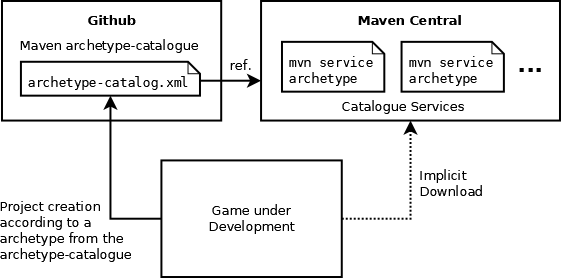
\includegraphics[width=12cm]{images/architecture/ServiceCatalogue}
	\caption{Integration of the service catalogue in \og{} development.}
	\label{fig:service_catalogue}
\end{figure}

The mostly used \ms{} of the service catalogue is the ``Hello World''
service which provides the means of bringing up a new \ms{} quickly.

\subsubsection{Consistency Requirements}

Consistency is a big concern in any distributed application and \ogs{} are no
exception. Consistency requirements for \ogs{} has already been researched in
project thesis one \todo{5.4 Non-functional requirements} and have been further
examined in this semester.

For \ogs{} consistency requirements can be categorized into strong consistency
for sensitive data like account or payment information and eventual consistency
for all other non critical game data. 

The final solution to consistency in MicroNet emphasises exactly this two
requirements. For transaction which require strong consistency it is aways
necessary that one single \ms{} maintains the overall control over the complete
transaction. This service then must use the underlying relational database to
make the transaction ACID by using the two phase commit protocol offered by the
database which is ProstgreSQL for MicroNet. This approach is mainly chosen due
to the reason that ACID transaction using eventual consistency are hard to get
right and therefore are error-prone \cite{zhang2011transaction},
\cite{zhang2008persistence}, and \cite{pardon2014atomic}.

For best effort consistency requirements eventual consistency is a solution that
has proven to work \cite{graham2016distributed_transactions}. Eventual
consistency emphasis scaling and robust systems in general. The drawback is the
added effort during development to implement a eventual consistent application.

Eventual consistency in MicroNet is realized by time-outs and retries. This is
realized by using the presistence system of the message broker in conjunction
with the request response functionality offered by MicroNet messaging. \mss{}
are advised to retry a transaction for a number of times\footnote{Five retries
seemed appropriate for most requests.}. If all retries where failures the
service must persistently log the unprocessed transaction and send an
informative message to the user. Over time the number of unprocessed transaction
should decrease. Unprocessed transaction can then be examined by developers in a
batch to find flaws in the application design.
developers

\subsection{Session Management}

MicroNet provides session management as a high level feature to tackle the
integral part of session handling in a \og{}. Player sessions are essential to
track actions of individual players and persist the progress of a player. Game
sessions tackle the issue that \ogs{} are state-full and therefore game session
in simulation services are unique. 

Session management has been one major issue throughout thesis one, two and
three. The final solution for session management relies on a NoSQL database.




\subsubsection{Player Sessions}

The authentication process that has briefly been mentioned in
\autoref{sub:networking} is responsible to establish player sessions. Once
authenticated player sessions can be used to collate incoming messages to users.
Player sessions can also be used to store frequently changing player data to
allow fast and global access. In MicroNet the player sessions can be accessed
through Couchbase.

One drawback that player session introduce is the fact that multiple API
gateways each gateway needs the ability to look-up player connections to
determine if the corresponding user is authenticated. This process has to be
done upon every player message which leads a lot of access to NoSQL. Another
possibility would be that the user needs to send a authentication cookie with
every message. This method introduces significant bandwidth overhead which is
worse. 

\begin{figure}
	\centering
  	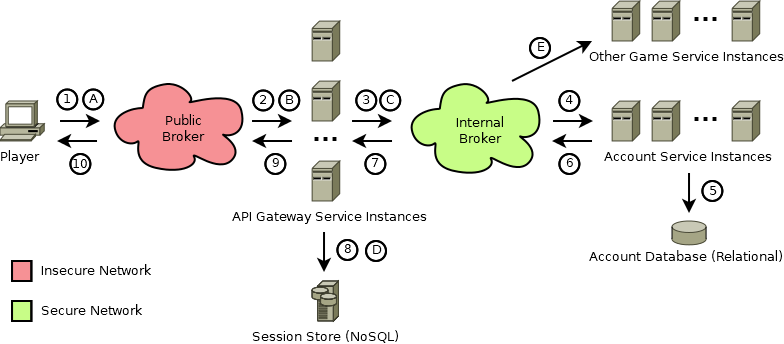
\includegraphics[width=\textwidth]{images/architecture/PlayerSessions}
	\caption{Player session authentication process.}
	\label{fig:player_sessions}
\end{figure}

\autoref{fig:player_sessions} shows the whole authentication process with the
result of a established authenticated player connection. The message flow
consists of the following steps:

\begin{enumerate}
  \item The user sends a login request to the public broker.
  \item One API Gateway polls the message in a competing consumer fashion.
  \item The gateway forwards the login message to the internal broker using the
  mn://account/login queue.
  \item One Account Service polls the message in a competing consumer fashion.
  \item The Account Service authenticates the user using the Account Database.
  \item The account service returns the login response to a temporary queue held
  open by the responsible gateway.
  \item The gateway service consumes the login response from the temporary
  queue.
  \item Upon login success the gateway adds a new player session to the session
  store, identified by the player connection.
  \item The gateway returns the login response to a temporary queue held open by
  the requesting player.
  \item The player consumes the login response from a temporary queue. Upon
  success he gains access to the game services (A, B, C, D\footnote{In step D
  the API Gateway must verify if the player connection is already
  authenticated. If the player is not authenticated no messages are forwarded.},
  E).
\end{enumerate}



\subsubsection{Game Sessions}

Game sessions are a strategy to deal with the state-fullness of \ogs{}. Game
sessions are unique and a player can only be in one game session at a time. Game
sessions are either infinitely or terminate at specific conditions. Either way
the player must be able to find the correct simulation instance which hosts the
game session he wants to participate in. MicroNet provides this functionality
through the WorldService which is part of the service catalogue.

\begin{figure}
	\centering
  	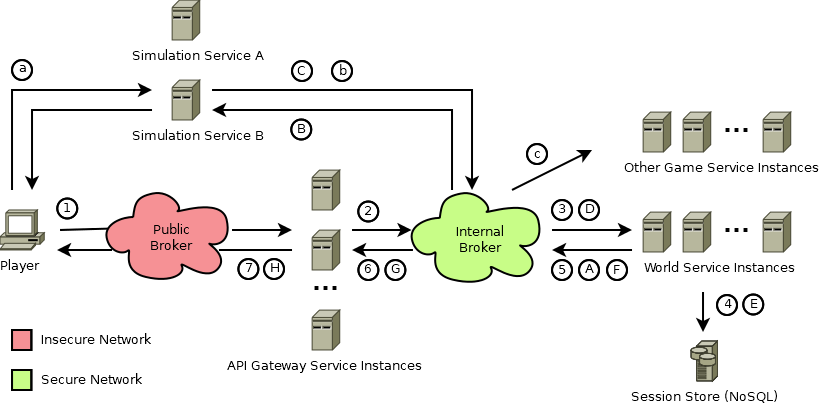
\includegraphics[width=\textwidth]{images/architecture/GameSessions}
	\caption{The join process of a game session.}
	\label{fig:game_sessions}
\end{figure}

\autoref{fig:game_sessions} shows the process how a game session is joined.
The join process consists of the following steps:

\begin{enumerate}
  \item The player sends a join request for game session B to the API gateway
  via the public message broker.
  \item The gateway service forwards the message to the mn://world/join queue
  via the internal message broker.
  \item One world service polls the message in a competing consumer fashion
  \item The world service checks is the session already exists in the session
  store. If not, the world service adds the game session to the session store,
  marks it as \textit{isOpening} and initiates the game session opening process (capital
  letter sequence in \autoref{fig:game_sessions}). In this case or if the
  session is currently opening the world service adds the player to a waiting
  queue for the session.
  \item If the game session is open the world service directly
  forwards the IP/Port combination to the player.  In this case the session is
  not open or opening a ``please wait'' response is forwarded to the player.
  \item The join response is consumed by a temporary queue held open by the API
  Gateway. The gateway forwards the join response to the player via the public
  broker.
  \item The player consumes the join response using a temporary queue. In the
  case the session was already open, the player can join right away. The regular
  session flow (a, c, c, \ldots) starts now.
\end{enumerate}

In the case the requested game session is not open when the player wants to
join\footnote{It is a common case that the game session is not open, for
example when the \og{} has many (thousands) of available game sessions.} the
session must be started asynchronously and the player must be notified when the
session is ready. This process consists of the following steps:



\begin{enumerate}[label=\Alph*.]
    \item The World Service sends an open region request to the
    mn://instance-open queue.
    \item One free simulation instance polls the open request in a competing
    consumer fasion.
    \item Once the simulation service is up and running, sends a simulation
    instance ready to the mn://world/instance/ready queue via the internal
    message broker.
    \item One World Service polls the instance ready message in a competing
    consumer fashion.
    \item The World Service marks the game session as \textit{isOpen} in the
    session store.
    \item The World service sends a broadcast event request to the
    mn://gateway/broadcast/event queue containing the IP/Port combination of the
    simulation service, addressed to all player is the waiting queue of the game
    session.
    \item One API Gateway polls the broadcast requests in a competing consumer
    fashion
    \item The Gateway broadcasts the join event to all waiting players. From
    then on the regular session flow (a, c, c, \ldots) starts.
\end{enumerate}





\subsection{MicroNet Tools}
\label{sub:tools}

The MicroNet tools are a collection of Eclipse plug-ins. Eclipse was chosen due
to the primary Java nature of MicroNet. This allows a quick development of Java
\mss{}. But the MicroNet tools also offer a way to integrate other
technologies into a \ms{} application. This language independence is
accomplished by using \gls{json} as a low level information exchange format. As
long as a technology supports \gls{json} it can participate in the application.
Another requirement is that it is possible to access to the message broker with
the foreign technology.

Since the \gls{ui} of an Eclipse plug-in is written using the Swing
Window Toolkit (SWT) library it can easily be exported to be a stand-alone tool
decoupled from Eclipse. With this approach it is possible to port the MicroNet
Tools to other platforms as long as they support a \gls{jvm}.

The MicroNet Tools have been completely developed within this last semester
thesis and are a major contribution to four of the hypotheses listed in
\autoref{sub:hypothesis}: the composition, deployment, simple development, and 
reproducibility hypotheses.

More information on the MicroNet Tools can be found in the MicroNet online
documentation \cite{micronet2017doku}.

\subsubsection{Files and Folders Structure}

To allow loose coupling of a \ms{} application MicroNet makes a few assumptions
on how to organize files and folders:

\begin{itemize}
  \item The eclipse workspace folder must contain one project folder for each
  \ms{}.
  \item For automated integration of a \ms{} its project folder must be either a
  Java/Maven project or it must contain a Dockerfile.
 \item One shared folder must be present to exchange the \textit{Shared Model} and the
  \textit{Service API}.
\end{itemize}  

\begin{figure}
	\centering
	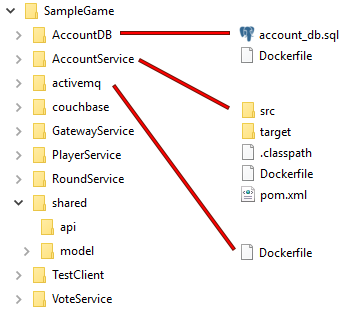
\includegraphics[width=9cm]{images/tools/folder_structure}
	\caption{Example folder structure of a MicroNet application workspace.}
	\label{fig:folder_structure}
\end{figure}

\autoref{fig:folder_structure} shows an example of a folder structure of a
MicroNet application workspace. The shared folder in this case is simply a folder within the
workspace. The figure also shows three canonical examples of project folders.
The AccountDB folder represents a containerized PostgreSQL database. The
AccountService folder is a standard MicroNet Maven/Java service project. The
activemq folder contains only a Dockerfile, which is the minimal requirement to
participate in a MicroNet application.

\subsubsection{Annotations}

MicroNet \textit{Annotations} provide a solution to define a \ms{} in a very
lean way. A service is defined by annotating an arbitrary class in the service
projects with the \textit{@MessageService(uri=``mn://service\_name'')}
\textit{Annotation}. Within the service class listener methods can be annotated
with the \textit{@MessageListener(uri=``/api\_method'')} \textit{Annotation} to
define the reactive behaviour of the service according to the defined \gls{api}.
Examples of services defined by the \textit{Annotation} can be seen in
\autoref{lst:service_communication} and \autoref{lst:message_parameters}.

\begin{figure}
\begin{lstlisting}[language=Java,firstnumber=1] 
@MessageService(uri = "mn://foo")
public class ServiceFoo {
	@OnStart
	public void onStart(Context context) {
		System.out.println("Start called");
	}
	
	@OnStop
	public void onStop(Context context) {
		System.out.println("Stop called");
	}
	
	@MessageListener(uri="/hello")
	@RequestPayload(UserValues.class) 
	@ResponsePayload(CredentialValues.class)
	@RequestParameters({
		@MessageParameter(code=ParameterCode.ID, type=Integer.class),
		@MessageParameter(code=ParameterCode.NAME, type=String.class)
	})
	@ResponseParameters({
		@MessageParameter(code=ParameterCode.ID, type=Integer.class),
	})
	public Response helloHandler(Context context, Request request) {
		int idParameter = request.getParameters().getInt(ParameterCode.ID);
		String nameParameter = request.getParameters()
			.getString(ParameterCode.NAME);
		
		UserValues user = Serialization.deserialize(
			request.getData(), UserValues.class);
		System.out.println("Process: " + user + " and " + nameParameter);

		String responseData = Serialization.serialize(user.getCredentials());
		Response response = new Response(StatusCode.OK, responseData);
		response.getParameters().set(ParameterCode.ID, idParameter);
		return response;
	}
}
\end{lstlisting}
\caption{A fully defined MicroNet \ms{} including all possible pre- and
post-condition \textit{Annotations}.}
\label{lst:pre_post_conditions}
\end{figure}

MicroNet \textit{Annotations} also provide a basic implementation of the design
by contract pattern. A service defines preconditions on request payloads and
defines post-conditions on response payloads. This system aims to prevent
semantic errors in communications. The pre- and post-conditions build the
foundation of the \textit{Code Assist} tool of MicroNet which helps the
developer in preventing mistakes in \ms{} communication design.
\autoref{lst:pre_post_conditions} shows a \ms{} defined by \textit{Annotations}
containing a well defined message listener with all pre- and post-conditions.
Theoretically the \textit{@RequestParameter} and \textit{@ResponseParameter}
\textit{Annotations} could implicitly be generated by parsing the \gls{ast} of
the listener method. This is however a very advanced topic which could fill a
whole thesis in itself.
 
 \paragraph{Annotation Processing}
 
Java annotations can either be used during run-time or processed during
compilation-time. MicroNet only processes \textit{Annotations} at compile-time.
Since Java version 6 the annotation processing process is tightly integrated
into the standard Java build process. This renders the \textit{Annotation}
process platform independent and it can be reproduced in a command line java
build, a Maven build or an Eclipse build\footnote{Annotation processing is
executed by the Java compiler which behaves slightly different for all evaluated
build setups (Eclipse, Maven, or Java native). Specifically newly generated
annotations are only found by the Eclipse proprietary compiler.}.

\textit{Annotation Processing} is also the entry point for code generation.
Even if no annotations are present in a project \textit{Annotation Processing}
can still be activated just to generate the \textit{Shared Model} and without
generating any service implementation. The MicroNet \textit{Annotation
Processor} provides an option for this purpose.

\subsubsection{Code Generation}

Code generation allows the developer to omit the boiler plate code that is
needed to integrate a service into a MicroNet application. This covers the setup
of the appropriate networking solution according to the environment and the
generation of the executable class of the \ms{}. This simplification allows the
developer to focus more on the actual domain logic of the \ms{}. It also spares
the developer having to register the main service class within the
application. The service class is automatically found and registration is
implicitly done by the \textit{Annotation Processor}.

The code generation library of MicroNet is very small and can be translated to
other programming languages very easily if needed. Since code generation is
basically nothing more than generating the right ``text-files'' this can be
accomplished in almost any imaginable programming language.

The MicroNet code generation library is implemented using the Java Poet
library. Java Poet allows for typesafe generation of Java classes and is very
easy to use. 

\paragraph{Service Generation}

The \textit{@MessageService} and \textit{@MessageListener} \textit{Annotations}
are used to build the executable class of a \ms{}. The executable class
registers all message listeners within the networking system. In addition the
annotated \textit{@Start} and \textit{@Stop} methods are called at service start
or at service termination respectively. The generated main method encompasses
the start/stop functionality and the listener registration in a defined set-up
sequence. \autoref{lst:generated_service} shows the generated implementation of
the annotated service shown in \autoref{lst:pre_post_conditions}.

\begin{figure}
\begin{lstlisting}[language=Java,firstnumber=1] 
public final class ServiceImpl {
  public static void main(String[] args) {
    try {
      System.out.println("Starting ServiceFoo...");

      IPeer peer = PeerFactory.createPeer();
      Context context = new Context(peer, "mn://foo");
      ServiceFoo service = new ServiceFoo();

      System.out.println("Registering message listeners...");
      peer.listen("/hello", (Request request) -> 
      	service.helloHandler(context, request));

      System.out.println("ServiceFoo started...");
      service.onStart(context);

      Runtime.getRuntime().addShutdownHook(new Thread() {
        @Override
        public void run() {
          System.out.println("ServiceFoo stopped...");
          service.onStop(context);
        }
      });
    }
    catch (Exception e) {
      System.err.println("Could not start ServiceFoo...");
      e.printStackTrace();
    }
  }
}
\end{lstlisting}
\caption{An executable \ms{} main class generated out of an annotated service
class.}
\label{lst:generated_service}
\end{figure}

\paragraph{Model Generation}

The model generation process is completely independent from the service
generation and is used to translate the game model which is defined in
\gls{json} to java POJOs (plain old Java objects). Because the MicroNet Model
generation library is very small it can also be reproduced in other programming
languages with relative ease. \autoref{lst:generated_model_class} shows the
\textit{UserValues} POJO generated out of the corresponding \textit{Template Type}
shown in \autoref{lst:template_type}.

\begin{figure}
\begin{lstlisting}[language=Java,firstnumber=1] 
public class UserValues {
  private int id;
  private CredentialValues credentials;

  public void setId(int id) {
    this.id=id;
  }

  public int getId() {
    return id;
  }

  public void setCredentials(CredentialValues credentials) {
    this.credentials=credentials;
  }

  public CredentialValues getCredentials() {
    return credentials;
  }
}
\end{lstlisting}
\caption{The UserValues POJO created out of the corresponding \textit{Template Type}.}
\label{lst:generated_model_class}
\end{figure}

The challenge for model generation is not the generation process itself but the
definition and editing process of the model that is generated and its
representation. These aspects make up a much larger part of MicroNet than the
actual code generation. Model editing and representation is further discussed
below in the paragraph on the \textit{Model Editor}.

\subsubsection{Code Assist}

The \textit{Code Assist} plug-in helps the developer to keep track of
functionality provided by other services. It presents the \textit{Service API}
in a type-safe way to the developer by relying on the pre- and postconditions
defined by MicroNet \textit{Annotations}.

\textit{Code Assist} is implemented by using the Eclipse code-completion
extension point. This extension point is used to add custom entries to the code
completion list box. This functionality is used to offer the MicroNet \gls{api}
to the developer any time he types \textit{``mn://''} in a source file. The
proposals are filtered according to the developer's input.

Type-safety enforcement is currently not implemented in MicroNet due to the same
reason as mentioned above in the section on \textit{Annotations} that require
parsing the \ms{} code. It could however be implemented by searching the
\gls{ast} of a message handler method for references on the request and response
objects. Calls to \code{getParameters()} or \code{setParameters()} can be
analyzed in regard to which \code{ParameterCode}s are used and which the
\textit{Template Type} of the parameter is. This feature would allow the
developer to omit the \code{@RequestParameters} and \code{@ResponseParameters}
\textit{Annotations}.

Upon violation of the message types the compiler can generate an error which
forces the developer to fix the issue before a build can be executed.
Although this process is possible the implementation of violation detection
again involves parsing the Java \gls{ast} and this effort is out of the scope of
this thesis.

In the current version of MicroNet the types are presented to the developer via
a tool-tip. Although type-safety is not enforced the developer can at least read
the correct types in the \textit{Code Assist} tool-tip, which alone is already
very helpful. \autoref{fig:code_assist} shows the \textit{Code Assist} tool-tip
for the \code{mn://foo/hello} message listener that was shown in 
\autoref{lst:pre_post_conditions}.

\begin{figure}
	\centering
	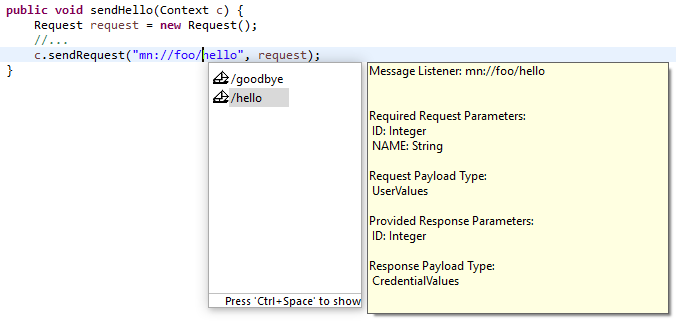
\includegraphics[width=\textwidth]{images/tools/CodeAssist}
	\caption{MicroNet \textit{Code Assist} tool-tip.}
	\label{fig:code_assist}
\end{figure}

\subsubsection{Service Explorer}

The \textit{Service Explorer} is the central management UI of a MicroNet and
helps the developer to get an overview over the whole game application. The
\textit{Service Explorer} is realized using a custom Eclipse view. The view
contains a list of all services showing their versions along with other useful
information like required ports or links to other services. The \textit{Service
Explorer} displays services which are Java, Maven and Docker projects. The
service list is dynamic and automatically refreshed when projects are created or
deleted.

The service list can be used to quickly edit the configuration of services. This
includes the port configuration as well as service linkage for the Docker
overlay network.

The \textit{Service Explorer} is also used to configure the composition of the
application in a visual way. Services can be activated to be part of the build
process, which automatically integrates them into the composition files (Maven:
pom.xml, Docker: docker-compose). This is done by deciding for each service
individually if it is part of the Maven build and/or part of the Docker
container build process.

The \textit{Service Explorer} also provides a quick interface to all launch
configurations explained in the \textit{Launch Utility} section below. The launch
functionality is provided with a context menu for each service in the list and
through the local pull-down menu offered by the Eclipse view.
\autoref{fig:service_explorer} shows the \textit{Service Explorer} with the
launch menu of the \code{FooService} open.

\begin{figure}
	\centering
	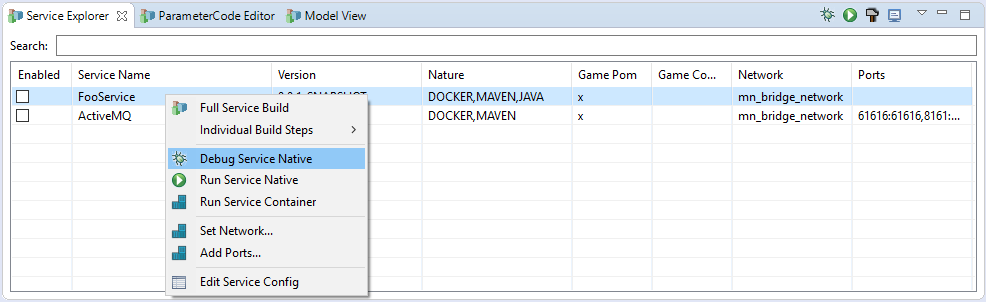
\includegraphics[width=\textwidth]{images/tools/ServiceExplorer}
	\caption{MicroNet \textit{Service Explorer}}
	\label{fig:service_explorer}
\end{figure}

\subsubsection{Launch Utility}

The \textit{Launch Utility} brings order to the vast different possibilities of
how to orchestrate a \ms{} application with containers. Many different configurations
can be helpful to develop, test and deploy a \ms{} application. The MicroNet
launch tools provide an easy way to set-up and start launch configurations.

The launch configurations of a Java/Maven build are offered via the Eclipse
Launcher plug-in. For these configurations the MicroNet \textit{Launch Utility}
only has to run the respective Eclipse Launch configuration.

Automation of the Docker container build process is not as simple because
Eclipse does not offer built-in functionality to access the Docker daemon.
The Docker Tools for Eclipse can be used to fulfill this gap since it provides
the necessary Docker container launch configurations. This however introduces a
strong dependency on the Docker Tools, which is undesirable. Many client for the
Docker daemon exist to integrate Docker automation into applications. This
however introduces another dependency closely related to Eclipse; and also the
tested Spotify Docker client which looks very promising has caused several class
path run-time errors and does not support Docker compose.

A workaround is to automate the Docker CLI using the Java run-time environment.
With this approach the docker commands are simply executed on the host of the
\gls{jvm}. This decouples the Docker integration mainly from Eclipse and places
it into the used Docker CLI. A Docker CLI is available for all major platforms:
Linux, Windows and MacOS. Since the docker CLI commands are the same on all
systems this is a platform independent approach since it only relies on a
\gls{jvm} and the docker CLI which is installed alongside Docker anyway. A
Drawback is that the developer has to configure the host-path to the docker CLI
executables. This is further complicated when Docker Toolbox instead of native
Docker is used since Docker Toolbox requires setting several Docker environment
variables. The MicroNet \textit{Launch Utility} however encompasses all this
functionality.

The \textit{Launch Utility} can deploy MicroNet applications in three distinct ways which
can all be combined which each other: local native, local containerized, and
cloud containerized. \autoref{fig:launch_utility} shows how the launch
configurations can be started via the \textit{Service Explorer}. The rest of this
paragraph explains all three deployment modes.

\begin{figure}
	\centering
	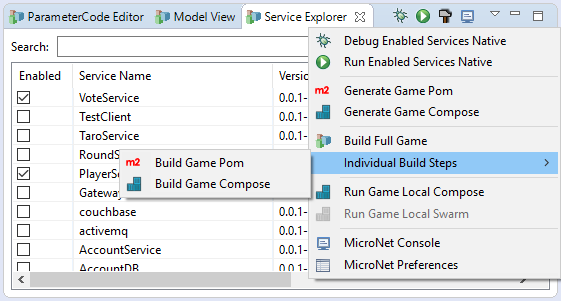
\includegraphics[width=14cm]{images/tools/LaunchUtility}
	\caption{\textit{Launch Utilities} offered by the \textit{Service Explorer}}
	\label{fig:launch_utility}
\end{figure}

\paragraph{Local Native}

\begin{figure}
	\centering
	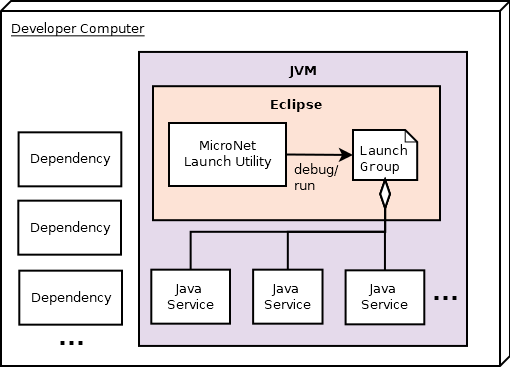
\includegraphics[width=10cm]{images/architecture/DeploymentLocalNative}
	\caption{Local native deployment of a MicroNet driven application.}
	\label{fig:deployment_local_native}
\end{figure}

The native configuration runs or debugs a game application as a set of native
Java applications. This makes debugging very fast and the integration in Eclipse
provides many useful debugging tools. To launch multiple Java applications at
once the CDT Launch Group plug-in is used. It composes multiple launch
configurations into a single configuration. Upon Launch Group execution all
contained applications are individually started. No build step is further needed
for this configuration.

For native configurations it is easiest to run software on which the application
depends as stand-alone installations on the host. Since the native configuration
is solely used during development this also allows the dependencies to be tested
isolated from the composed application. It is nonetheless possible to combine a
local native configuration with a local containerized configuration. Services
and dependencies can therefore be started in the configuration best suited for
them.

\autoref{fig:deployment_local_native} shows the deployment of a MicroNet
driven game in local deployment mode.

\paragraph{Local Containerized}

The local containerized configuration is meant to reproduce the final deployment
process on the local developer machine. For this purpose Maven and Docker
compose/swarm are used. 

A local Maven build of the complete application is done by aggregating the
individual Maven service projects into a master .pom file. The master .pom can
be used to build the whole application at once. The kind of services that are
aggregated to the master .pom file can be configured via. the \textit{Service Explorer}.

A local Docker deployment is defined by a docker-compose file. This file is also
defined by configuring services via the \textit{Service Explorer}. The Docker build
process is then simply invoked by building the docker-compose file.

In order to run the local containerized application the local docker engine can
be used. Docker-compose is natively installed with most docker installations or
can be separately installed. The application can be started locally either using
Docker-compose or docker swarm commands. On the local developer machine there is
only little difference between docker-compose and -swarm. Networking however
behaves differently locally and in the cloud so the local networking
configuration cannot be identically transferred to the cloud environment.

\begin{figure}
	\centering
	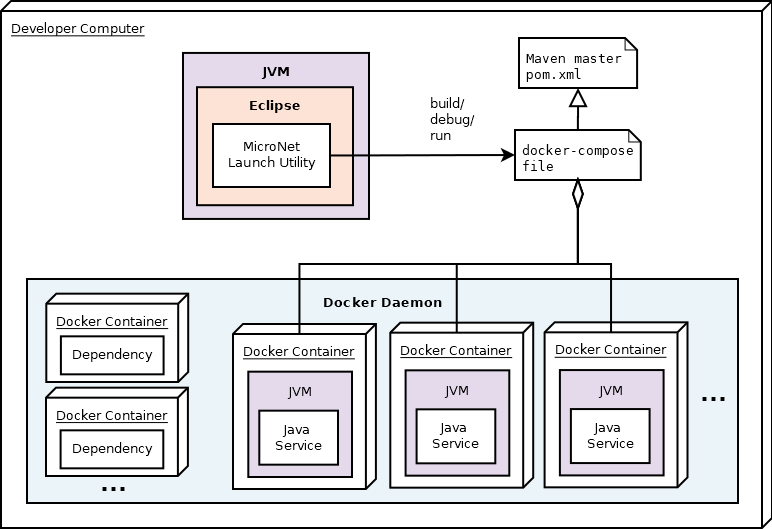
\includegraphics[width=\textwidth]{images/architecture/DeploymentLocalContainerized}
	\caption{Local containerized deployment of a MicroNet driven application.}
	\label{fig:deployment_local_containerized}
\end{figure}

\autoref{fig:deployment_local_containerized} shows how an application is
composed and deployed in the local containerized mode.

\paragraph{Cloud Containerized}

The final step of \ms{} application deployment is cloud deployment. The idea
behind application containerization is that this process is meant to be
deterministically reproducible on different systems. Therefore if the
application is working in the local containerized configuration the cloud
configuration can be achieved in a similar way.

MicroNet does not provide any out-of-the box solution to automatically deploy an
application in the cloud. This is because of the variety of
different infrastructures that can be used to deploy MicroNet. But the
deployment is prepared by MicroNet so it can be done with very few console
commands via SSH.

Due to the restrictions mentioned in \autoref{sub:zero_buget} the production
environment of \mn{} is a virtual Linux server in the HSR cloud. The cloud
deployment process is mainly based on this environment. Since this a very
general setup the process can easily be reproduced on other environments.

In order to deploy a MicroNet \ms{} application the developer must perform the
following steps under the assumption that the server runs a fresh Linux
installation.

\begin{itemize}
  \item Install: Docker Engine, Java, Maven and Git.
  \item Initialize docker swarm (master and worker machines).
  \item Pull the game application repository via Git (containing all service
  projects and the shared folder).
  \item Build the application class files using the master .pom file (annotation
  processing and code generation is performed during this step).
  \item Containerize the application using docker-compose \gls{api} and the generated
  docker-compose file.
  \item Launch the application in Docker Swarm using the docker stack \gls{api}.
\end{itemize}

\begin{figure}
	\hspace*{-0.8cm}
	\centering
	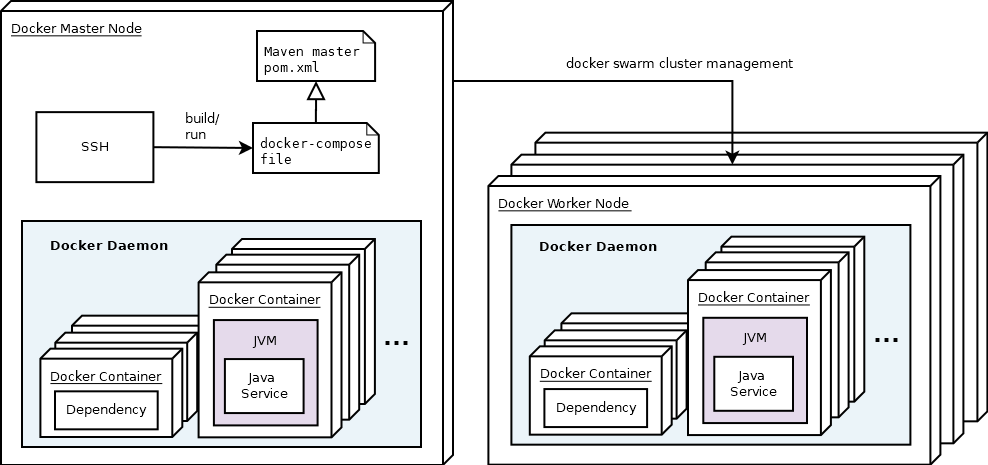
\includegraphics[width=1.1\textwidth]{images/architecture/DeploymentCloudContainerized}
	\caption{Cloud containerized deployment of a MicroNet driven application.}
	\label{fig:deployment_cloud_containerized}
\end{figure}

This sounds like a lot of steps but in fact the process is reasonably quick and
only requires very few console commands which can be looked up in the MicroNet
documentation \cite{micronet2017doku}.
\autoref{fig:deployment_cloud_containerized} gives an impression on how such a
docker-swarm environment may look like.

\subsubsection{Model Editor}

The \textit{Model Editor} is the last feature that was introduced in MicroNet
tools. It is the final solution for how to cope with logical \ms{} composition
through the \textit{Shared Model} in a visual way. Since the game model is
designed to be mainly machine-readable it is not suited to be directly edited in
the underlying \gls{json} files. The \textit{Model Editor} is designed to allow
convenient defining and editing of the model in a way which is especially useful
for \og{} application.

The \textit{Model Editor} is basically a graph editor visualizing a direct
representation of the game graph to allow extending and changing the graph. The
graph has three root nodes each of which span a model tree: the parameter code
list, the \textit{Template Tree}, and the \textit{Prefab Tree}.

\paragraph{Parameter Code List}

The parameter code tree is simply a flat list of String constants which define
all the parameter codes used throughout the application. This global approach
allows the substitution of the parameter codes strings with numbers, which is
more space efficient. Since parameters are used very often this has a noticeable
impact on the bandwidth requirements of an application.

\paragraph{Template Tree}

The \textit{Template Tree} allows to edit the game's \textit{Template Types}
using graph editing. Object Types defined using the \textit{Template Tree} can
be used for message transfer and persistence. \textit{Template Type} are
descriptions of domain objects and are used to generate \textit{Shared Model}
classes (POJOs) during code generation.

A \textit{Template Type} consists of a set of fields that may be of the
following types: STRING, NUMBER, BOOLEAN, CHAR, ENUM, LIST, SET, MAP, and
COMPONENT. The types are derived from the Java types since they are well
documented and can be redefined in other programming languages using the Java
language specifications.

The COMPONENT type can be any other \textit{Template Type}. A component is
represented as a field in the data class. Also \textit{Template Types} can be
derived from other \textit{Template Types}. The derivation is realized using
regular Java inheritance. \autoref{fig:model_view} shows the \textit{Model
Editor} which can be used to manually edit the \textit{Template Tree}.

\begin{figure}
	\centering
	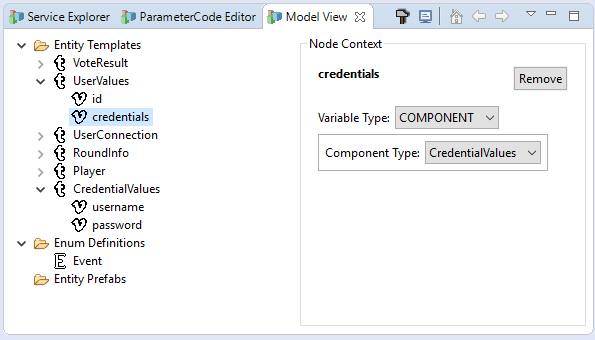
\includegraphics[width=\textwidth]{images/tools/ModelView}
	\caption{\textit{Template Type} editing with the MicroNet \textit{Model Editor}.}
	\label{fig:model_view}
\end{figure}

\paragraph{Prefab Tree}

The \textit{Prefab Tree} is a ``physical'' instantiation of the game graph. It
contains actual instances of \textit{Template Types}. This can be used by game
designers to pre-define game objects that are later used in the game. The
\textit{Prefab Tree} is directly compatible with the serialization component
provided by MicroNet. The generated model classes which represent the
\textit{Template Types} can be used to directly serialize and de-serialize game
objects which are part of the prefab-tree. The serialized data can directly be
stored in the database or be used as a payload or as parameters for message
transfers.

The \textit{Prefab Tree} can either be persisted in the file-system or persisted in the
database in \gls{json} format. The \textit{Prefab} approach allows for very
convenient and consistent handling of game data both during development and
operation.


\subsection{Example Game}

MicroNet provides a simple but complete example of an \og{}. Although the sample
game is very simple it gives a good overview over the functionality of MicroNet.

The sample game is a guessing game which is played in rounds of 15 seconds.
In each round the players have to guess a number between 1 and 100. The players
receive a score based on the proximity of the guess to the number. The score of
all player is shown in a scoreboard. 

The game client of the sample game is a standalone Java application using the
Laterna console gui library. Laterna allows to develop window based GUIs for the
terminal. This allows to run the game client also on server environments
through the command line. \todo{screenshot}

\autoref{fig:sample_game_flow} shows the communication of the sample game. The
numeric sequence is the communication flow of a player vote and the capital
letter sequence is the round control communication.\\

\begin{figure}
	\centering
	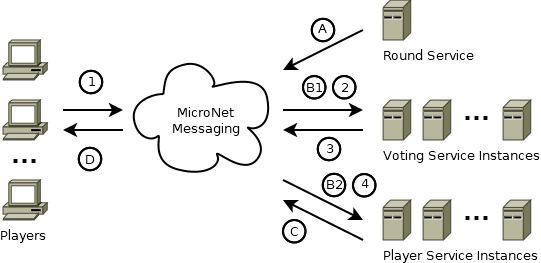
\includegraphics[width=\textwidth]{images/architecture/SampleGame}
	\caption{Communication flow of the Example Game.}
	\label{fig:sample_game_flow}
\end{figure}

The round control communication flow:

\begin{enumerate}[label=\Alph*.]
  \item The round service broadcasts a new new round event. The new round event
  contains the guessed number for the next round.
  \item \begin{enumerate}[label=\arabic*.]
    \item All voting services receive the new round event and store next the
    guess number in memory.
  	\item One player service receives the new round event to issue a score
  	broadcast. The scores of all players are available through the session store.
  \end{enumerate}
  \item The player service which received the new round event broadcasts a score
  update event to all participating players.
  \item Each player received the score update and updates its scoreboard
  accordingly.
   
\end{enumerate}

The player voting communication flow:

\begin{enumerate}
  \item The player sends his vote to the game application.
  \item The voting service instances compete for the vote messages.
  \item The processing voting service instance sends a score update message to
  an arbitrary player service.
  \item The processing player service persists the vote using the session store.
\end{enumerate}

It has to be mentioned that the round service is a singleton service. This is
necessary to ensure that the new round event is broadcast only once. Problems
like this are very common in distributed game development. To ensure the
stability of the application despite having singleton services can be quite a
challenge. One strategy is to keep singleton services as small as possible to
leave little room for failure. In the case of a failure the composition engine
must ensure that the singleton service is restarted. 

A singleton service must be designed in a way that no crucial data is lost upon
service failure and it must be possible to recover the state of a singleton
service after service failure.




\subsection{Testability}

The testing concept for \ms{} applications relies on the integrated in the
Maven build process of the application. Since the services expose their API as
Java functions testing can bypass networking for testing. The handler functions
are called directly in the test classes.

One problem with \ms{} testing is the access to the database. To spare the
developer with the need to mock the database a containerized database that can
be started before any tests are executed.
 

